% Created by tikzDevice version 0.10.1 on 2018-03-11 19:44:55
% !TEX encoding = UTF-8 Unicode
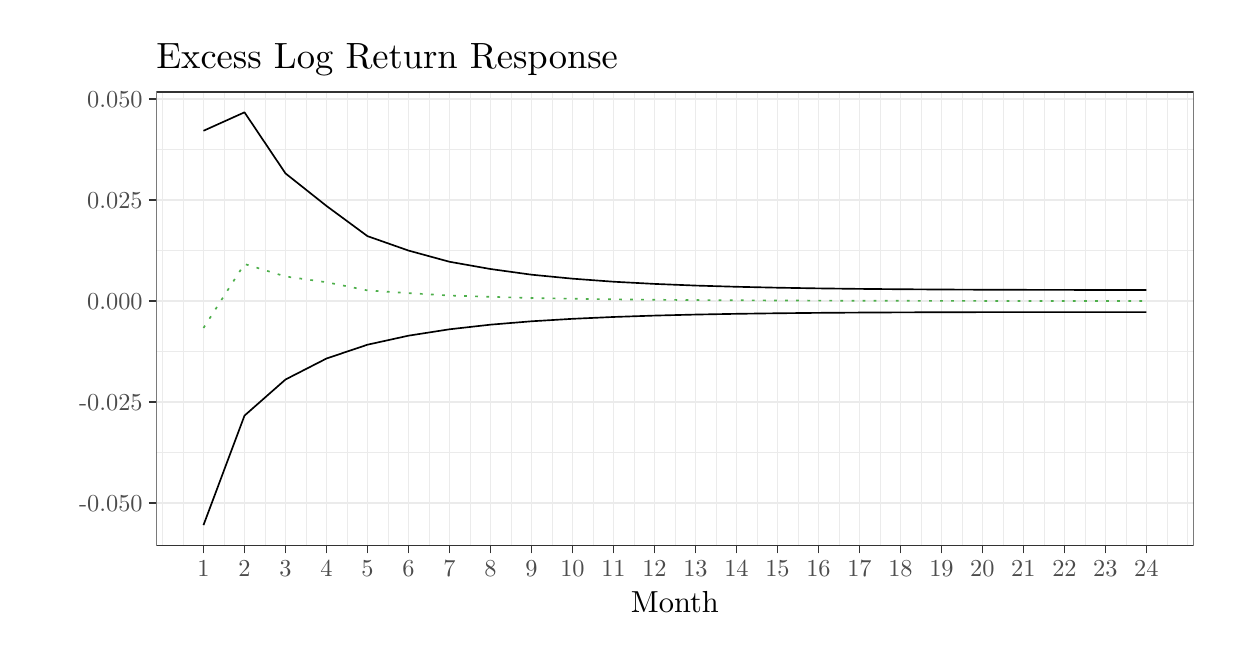
\begin{tikzpicture}[x=1pt,y=1pt]
\definecolor{fillColor}{RGB}{255,255,255}
\path[use as bounding box,fill=fillColor,fill opacity=0.00] (0,0) rectangle (426.79,216.81);
\begin{scope}
\path[clip] (  0.00,  0.00) rectangle (426.79,216.81);
\definecolor{drawColor}{RGB}{255,255,255}
\definecolor{fillColor}{RGB}{255,255,255}

\path[draw=drawColor,line width= 0.6pt,line join=round,line cap=round,fill=fillColor] (  0.00,  0.00) rectangle (426.79,216.81);
\end{scope}
\begin{scope}
\path[clip] ( 46.50, 29.59) rectangle (421.29,193.67);
\definecolor{fillColor}{RGB}{255,255,255}

\path[fill=fillColor] ( 46.50, 29.59) rectangle (421.29,193.67);
\definecolor{drawColor}{gray}{0.92}

\path[draw=drawColor,line width= 0.3pt,line join=round] ( 46.50, 63.32) --
	(421.29, 63.32);

\path[draw=drawColor,line width= 0.3pt,line join=round] ( 46.50, 99.79) --
	(421.29, 99.79);

\path[draw=drawColor,line width= 0.3pt,line join=round] ( 46.50,136.27) --
	(421.29,136.27);

\path[draw=drawColor,line width= 0.3pt,line join=round] ( 46.50,172.74) --
	(421.29,172.74);

\path[draw=drawColor,line width= 0.3pt,line join=round] ( 48.72, 29.59) --
	( 48.72,193.67);

\path[draw=drawColor,line width= 0.3pt,line join=round] ( 56.13, 29.59) --
	( 56.13,193.67);

\path[draw=drawColor,line width= 0.3pt,line join=round] ( 70.94, 29.59) --
	( 70.94,193.67);

\path[draw=drawColor,line width= 0.3pt,line join=round] ( 85.76, 29.59) --
	( 85.76,193.67);

\path[draw=drawColor,line width= 0.3pt,line join=round] (100.57, 29.59) --
	(100.57,193.67);

\path[draw=drawColor,line width= 0.3pt,line join=round] (115.38, 29.59) --
	(115.38,193.67);

\path[draw=drawColor,line width= 0.3pt,line join=round] (130.20, 29.59) --
	(130.20,193.67);

\path[draw=drawColor,line width= 0.3pt,line join=round] (145.01, 29.59) --
	(145.01,193.67);

\path[draw=drawColor,line width= 0.3pt,line join=round] (159.82, 29.59) --
	(159.82,193.67);

\path[draw=drawColor,line width= 0.3pt,line join=round] (174.64, 29.59) --
	(174.64,193.67);

\path[draw=drawColor,line width= 0.3pt,line join=round] (189.45, 29.59) --
	(189.45,193.67);

\path[draw=drawColor,line width= 0.3pt,line join=round] (204.27, 29.59) --
	(204.27,193.67);

\path[draw=drawColor,line width= 0.3pt,line join=round] (219.08, 29.59) --
	(219.08,193.67);

\path[draw=drawColor,line width= 0.3pt,line join=round] (233.89, 29.59) --
	(233.89,193.67);

\path[draw=drawColor,line width= 0.3pt,line join=round] (248.71, 29.59) --
	(248.71,193.67);

\path[draw=drawColor,line width= 0.3pt,line join=round] (263.52, 29.59) --
	(263.52,193.67);

\path[draw=drawColor,line width= 0.3pt,line join=round] (278.34, 29.59) --
	(278.34,193.67);

\path[draw=drawColor,line width= 0.3pt,line join=round] (293.15, 29.59) --
	(293.15,193.67);

\path[draw=drawColor,line width= 0.3pt,line join=round] (307.96, 29.59) --
	(307.96,193.67);

\path[draw=drawColor,line width= 0.3pt,line join=round] (322.78, 29.59) --
	(322.78,193.67);

\path[draw=drawColor,line width= 0.3pt,line join=round] (337.59, 29.59) --
	(337.59,193.67);

\path[draw=drawColor,line width= 0.3pt,line join=round] (352.41, 29.59) --
	(352.41,193.67);

\path[draw=drawColor,line width= 0.3pt,line join=round] (367.22, 29.59) --
	(367.22,193.67);

\path[draw=drawColor,line width= 0.3pt,line join=round] (382.03, 29.59) --
	(382.03,193.67);

\path[draw=drawColor,line width= 0.3pt,line join=round] (396.85, 29.59) --
	(396.85,193.67);

\path[draw=drawColor,line width= 0.3pt,line join=round] (411.66, 29.59) --
	(411.66,193.67);

\path[draw=drawColor,line width= 0.3pt,line join=round] (419.07, 29.59) --
	(419.07,193.67);

\path[draw=drawColor,line width= 0.6pt,line join=round] ( 46.50, 45.08) --
	(421.29, 45.08);

\path[draw=drawColor,line width= 0.6pt,line join=round] ( 46.50, 81.56) --
	(421.29, 81.56);

\path[draw=drawColor,line width= 0.6pt,line join=round] ( 46.50,118.03) --
	(421.29,118.03);

\path[draw=drawColor,line width= 0.6pt,line join=round] ( 46.50,154.50) --
	(421.29,154.50);

\path[draw=drawColor,line width= 0.6pt,line join=round] ( 46.50,190.98) --
	(421.29,190.98);

\path[draw=drawColor,line width= 0.6pt,line join=round] ( 63.53, 29.59) --
	( 63.53,193.67);

\path[draw=drawColor,line width= 0.6pt,line join=round] ( 78.35, 29.59) --
	( 78.35,193.67);

\path[draw=drawColor,line width= 0.6pt,line join=round] ( 93.16, 29.59) --
	( 93.16,193.67);

\path[draw=drawColor,line width= 0.6pt,line join=round] (107.98, 29.59) --
	(107.98,193.67);

\path[draw=drawColor,line width= 0.6pt,line join=round] (122.79, 29.59) --
	(122.79,193.67);

\path[draw=drawColor,line width= 0.6pt,line join=round] (137.60, 29.59) --
	(137.60,193.67);

\path[draw=drawColor,line width= 0.6pt,line join=round] (152.42, 29.59) --
	(152.42,193.67);

\path[draw=drawColor,line width= 0.6pt,line join=round] (167.23, 29.59) --
	(167.23,193.67);

\path[draw=drawColor,line width= 0.6pt,line join=round] (182.05, 29.59) --
	(182.05,193.67);

\path[draw=drawColor,line width= 0.6pt,line join=round] (196.86, 29.59) --
	(196.86,193.67);

\path[draw=drawColor,line width= 0.6pt,line join=round] (211.67, 29.59) --
	(211.67,193.67);

\path[draw=drawColor,line width= 0.6pt,line join=round] (226.49, 29.59) --
	(226.49,193.67);

\path[draw=drawColor,line width= 0.6pt,line join=round] (241.30, 29.59) --
	(241.30,193.67);

\path[draw=drawColor,line width= 0.6pt,line join=round] (256.12, 29.59) --
	(256.12,193.67);

\path[draw=drawColor,line width= 0.6pt,line join=round] (270.93, 29.59) --
	(270.93,193.67);

\path[draw=drawColor,line width= 0.6pt,line join=round] (285.74, 29.59) --
	(285.74,193.67);

\path[draw=drawColor,line width= 0.6pt,line join=round] (300.56, 29.59) --
	(300.56,193.67);

\path[draw=drawColor,line width= 0.6pt,line join=round] (315.37, 29.59) --
	(315.37,193.67);

\path[draw=drawColor,line width= 0.6pt,line join=round] (330.19, 29.59) --
	(330.19,193.67);

\path[draw=drawColor,line width= 0.6pt,line join=round] (345.00, 29.59) --
	(345.00,193.67);

\path[draw=drawColor,line width= 0.6pt,line join=round] (359.81, 29.59) --
	(359.81,193.67);

\path[draw=drawColor,line width= 0.6pt,line join=round] (374.63, 29.59) --
	(374.63,193.67);

\path[draw=drawColor,line width= 0.6pt,line join=round] (389.44, 29.59) --
	(389.44,193.67);

\path[draw=drawColor,line width= 0.6pt,line join=round] (404.26, 29.59) --
	(404.26,193.67);
\definecolor{drawColor}{RGB}{77,175,74}

\path[draw=drawColor,line width= 0.6pt,dash pattern=on 1pt off 3pt ,line join=round] ( 63.53,108.30) --
	( 78.35,131.42) --
	( 93.16,126.91) --
	(107.98,124.82) --
	(122.79,121.87) --
	(137.60,120.89) --
	(152.42,120.02) --
	(167.23,119.55) --
	(182.05,119.13) --
	(196.86,118.86) --
	(211.67,118.64) --
	(226.49,118.49) --
	(241.30,118.38) --
	(256.12,118.30) --
	(270.93,118.23) --
	(285.74,118.18) --
	(300.56,118.14) --
	(315.37,118.11) --
	(330.19,118.09) --
	(345.00,118.07) --
	(359.81,118.05) --
	(374.63,118.04) --
	(389.44,118.03) --
	(404.26,118.02);
\definecolor{drawColor}{RGB}{0,0,0}

\path[draw=drawColor,line width= 0.6pt,line join=round] ( 63.53, 37.05) --
	( 78.35, 76.63) --
	( 93.16, 89.67) --
	(107.98, 97.26) --
	(122.79,102.25) --
	(137.60,105.51) --
	(152.42,107.82) --
	(167.23,109.49) --
	(182.05,110.71) --
	(196.86,111.60) --
	(211.67,112.27) --
	(226.49,112.77) --
	(241.30,113.14) --
	(256.12,113.41) --
	(270.93,113.61) --
	(285.74,113.76) --
	(300.56,113.86) --
	(315.37,113.93) --
	(330.19,113.98) --
	(345.00,114.01) --
	(359.81,114.02) --
	(374.63,114.03) --
	(389.44,114.03) --
	(404.26,114.01);

\path[draw=drawColor,line width= 0.6pt,line join=round] ( 63.53,179.55) --
	( 78.35,186.22) --
	( 93.16,164.15) --
	(107.98,152.39) --
	(122.79,141.48) --
	(137.60,136.27) --
	(152.42,132.22) --
	(167.23,129.60) --
	(182.05,127.55) --
	(196.86,126.11) --
	(211.67,125.01) --
	(226.49,124.22) --
	(241.30,123.62) --
	(256.12,123.18) --
	(270.93,122.85) --
	(285.74,122.60) --
	(300.56,122.42) --
	(315.37,122.29) --
	(330.19,122.19) --
	(345.00,122.12) --
	(359.81,122.08) --
	(374.63,122.05) --
	(389.44,122.03) --
	(404.26,122.02);
\definecolor{drawColor}{gray}{0.20}

\path[draw=drawColor,line width= 0.6pt,line join=round,line cap=round] ( 46.50, 29.59) rectangle (421.29,193.67);
\end{scope}
\begin{scope}
\path[clip] (  0.00,  0.00) rectangle (426.79,216.81);
\definecolor{drawColor}{gray}{0.30}

\node[text=drawColor,anchor=base east,inner sep=0pt, outer sep=0pt, scale=  0.88] at ( 41.55, 42.05) {-0.050};

\node[text=drawColor,anchor=base east,inner sep=0pt, outer sep=0pt, scale=  0.88] at ( 41.55, 78.53) {-0.025};

\node[text=drawColor,anchor=base east,inner sep=0pt, outer sep=0pt, scale=  0.88] at ( 41.55,115.00) {0.000};

\node[text=drawColor,anchor=base east,inner sep=0pt, outer sep=0pt, scale=  0.88] at ( 41.55,151.47) {0.025};

\node[text=drawColor,anchor=base east,inner sep=0pt, outer sep=0pt, scale=  0.88] at ( 41.55,187.95) {0.050};
\end{scope}
\begin{scope}
\path[clip] (  0.00,  0.00) rectangle (426.79,216.81);
\definecolor{drawColor}{gray}{0.20}

\path[draw=drawColor,line width= 0.6pt,line join=round] ( 43.75, 45.08) --
	( 46.50, 45.08);

\path[draw=drawColor,line width= 0.6pt,line join=round] ( 43.75, 81.56) --
	( 46.50, 81.56);

\path[draw=drawColor,line width= 0.6pt,line join=round] ( 43.75,118.03) --
	( 46.50,118.03);

\path[draw=drawColor,line width= 0.6pt,line join=round] ( 43.75,154.50) --
	( 46.50,154.50);

\path[draw=drawColor,line width= 0.6pt,line join=round] ( 43.75,190.98) --
	( 46.50,190.98);
\end{scope}
\begin{scope}
\path[clip] (  0.00,  0.00) rectangle (426.79,216.81);
\definecolor{drawColor}{gray}{0.20}

\path[draw=drawColor,line width= 0.6pt,line join=round] ( 63.53, 26.84) --
	( 63.53, 29.59);

\path[draw=drawColor,line width= 0.6pt,line join=round] ( 78.35, 26.84) --
	( 78.35, 29.59);

\path[draw=drawColor,line width= 0.6pt,line join=round] ( 93.16, 26.84) --
	( 93.16, 29.59);

\path[draw=drawColor,line width= 0.6pt,line join=round] (107.98, 26.84) --
	(107.98, 29.59);

\path[draw=drawColor,line width= 0.6pt,line join=round] (122.79, 26.84) --
	(122.79, 29.59);

\path[draw=drawColor,line width= 0.6pt,line join=round] (137.60, 26.84) --
	(137.60, 29.59);

\path[draw=drawColor,line width= 0.6pt,line join=round] (152.42, 26.84) --
	(152.42, 29.59);

\path[draw=drawColor,line width= 0.6pt,line join=round] (167.23, 26.84) --
	(167.23, 29.59);

\path[draw=drawColor,line width= 0.6pt,line join=round] (182.05, 26.84) --
	(182.05, 29.59);

\path[draw=drawColor,line width= 0.6pt,line join=round] (196.86, 26.84) --
	(196.86, 29.59);

\path[draw=drawColor,line width= 0.6pt,line join=round] (211.67, 26.84) --
	(211.67, 29.59);

\path[draw=drawColor,line width= 0.6pt,line join=round] (226.49, 26.84) --
	(226.49, 29.59);

\path[draw=drawColor,line width= 0.6pt,line join=round] (241.30, 26.84) --
	(241.30, 29.59);

\path[draw=drawColor,line width= 0.6pt,line join=round] (256.12, 26.84) --
	(256.12, 29.59);

\path[draw=drawColor,line width= 0.6pt,line join=round] (270.93, 26.84) --
	(270.93, 29.59);

\path[draw=drawColor,line width= 0.6pt,line join=round] (285.74, 26.84) --
	(285.74, 29.59);

\path[draw=drawColor,line width= 0.6pt,line join=round] (300.56, 26.84) --
	(300.56, 29.59);

\path[draw=drawColor,line width= 0.6pt,line join=round] (315.37, 26.84) --
	(315.37, 29.59);

\path[draw=drawColor,line width= 0.6pt,line join=round] (330.19, 26.84) --
	(330.19, 29.59);

\path[draw=drawColor,line width= 0.6pt,line join=round] (345.00, 26.84) --
	(345.00, 29.59);

\path[draw=drawColor,line width= 0.6pt,line join=round] (359.81, 26.84) --
	(359.81, 29.59);

\path[draw=drawColor,line width= 0.6pt,line join=round] (374.63, 26.84) --
	(374.63, 29.59);

\path[draw=drawColor,line width= 0.6pt,line join=round] (389.44, 26.84) --
	(389.44, 29.59);

\path[draw=drawColor,line width= 0.6pt,line join=round] (404.26, 26.84) --
	(404.26, 29.59);
\end{scope}
\begin{scope}
\path[clip] (  0.00,  0.00) rectangle (426.79,216.81);
\definecolor{drawColor}{gray}{0.30}

\node[text=drawColor,anchor=base,inner sep=0pt, outer sep=0pt, scale=  0.88] at ( 63.53, 18.58) {1};

\node[text=drawColor,anchor=base,inner sep=0pt, outer sep=0pt, scale=  0.88] at ( 78.35, 18.58) {2};

\node[text=drawColor,anchor=base,inner sep=0pt, outer sep=0pt, scale=  0.88] at ( 93.16, 18.58) {3};

\node[text=drawColor,anchor=base,inner sep=0pt, outer sep=0pt, scale=  0.88] at (107.98, 18.58) {4};

\node[text=drawColor,anchor=base,inner sep=0pt, outer sep=0pt, scale=  0.88] at (122.79, 18.58) {5};

\node[text=drawColor,anchor=base,inner sep=0pt, outer sep=0pt, scale=  0.88] at (137.60, 18.58) {6};

\node[text=drawColor,anchor=base,inner sep=0pt, outer sep=0pt, scale=  0.88] at (152.42, 18.58) {7};

\node[text=drawColor,anchor=base,inner sep=0pt, outer sep=0pt, scale=  0.88] at (167.23, 18.58) {8};

\node[text=drawColor,anchor=base,inner sep=0pt, outer sep=0pt, scale=  0.88] at (182.05, 18.58) {9};

\node[text=drawColor,anchor=base,inner sep=0pt, outer sep=0pt, scale=  0.88] at (196.86, 18.58) {10};

\node[text=drawColor,anchor=base,inner sep=0pt, outer sep=0pt, scale=  0.88] at (211.67, 18.58) {11};

\node[text=drawColor,anchor=base,inner sep=0pt, outer sep=0pt, scale=  0.88] at (226.49, 18.58) {12};

\node[text=drawColor,anchor=base,inner sep=0pt, outer sep=0pt, scale=  0.88] at (241.30, 18.58) {13};

\node[text=drawColor,anchor=base,inner sep=0pt, outer sep=0pt, scale=  0.88] at (256.12, 18.58) {14};

\node[text=drawColor,anchor=base,inner sep=0pt, outer sep=0pt, scale=  0.88] at (270.93, 18.58) {15};

\node[text=drawColor,anchor=base,inner sep=0pt, outer sep=0pt, scale=  0.88] at (285.74, 18.58) {16};

\node[text=drawColor,anchor=base,inner sep=0pt, outer sep=0pt, scale=  0.88] at (300.56, 18.58) {17};

\node[text=drawColor,anchor=base,inner sep=0pt, outer sep=0pt, scale=  0.88] at (315.37, 18.58) {18};

\node[text=drawColor,anchor=base,inner sep=0pt, outer sep=0pt, scale=  0.88] at (330.19, 18.58) {19};

\node[text=drawColor,anchor=base,inner sep=0pt, outer sep=0pt, scale=  0.88] at (345.00, 18.58) {20};

\node[text=drawColor,anchor=base,inner sep=0pt, outer sep=0pt, scale=  0.88] at (359.81, 18.58) {21};

\node[text=drawColor,anchor=base,inner sep=0pt, outer sep=0pt, scale=  0.88] at (374.63, 18.58) {22};

\node[text=drawColor,anchor=base,inner sep=0pt, outer sep=0pt, scale=  0.88] at (389.44, 18.58) {23};

\node[text=drawColor,anchor=base,inner sep=0pt, outer sep=0pt, scale=  0.88] at (404.26, 18.58) {24};
\end{scope}
\begin{scope}
\path[clip] (  0.00,  0.00) rectangle (426.79,216.81);
\definecolor{drawColor}{RGB}{0,0,0}

\node[text=drawColor,anchor=base,inner sep=0pt, outer sep=0pt, scale=  1.10] at (233.89,  5.50) {Month};
\end{scope}
\begin{scope}
\path[clip] (  0.00,  0.00) rectangle (426.79,216.81);
\definecolor{drawColor}{RGB}{0,0,0}

\node[text=drawColor,anchor=base west,inner sep=0pt, outer sep=0pt, scale=  1.32] at ( 46.50,202.22) {Excess Log Return Response};
\end{scope}
\end{tikzpicture}
